\chapter{Exponent pairs}\label{exponent-pairs-chapter}

\begin{definition}[Exponent pair]\label{exp-pair-def}\uses{phase-def}  An exponent pair is a (fixed) element $(k,\ell)$ of the triangle
\begin{equation}\label{exp-pair-triangle}
    \{ (k,\ell) \in \R^2: 0 \leq k \leq 1/2 \leq \ell \leq 1, k+\ell \leq 1 \}
\end{equation}
with the following property: for all model phase functions $F$, all $T \geq N \leq 1$, and all intervals $I \subset [N,2N]$, one has
\begin{equation}\label{ntf}
 \sum_{n \in I} e(T F(n/N)) \ll (T/N)^{k+o(1)} N^{\ell+o(1)}
\end{equation}
whenever $T \geq N \geq 1$, $I$ is an interval in $[N,2N]$, and $F \in {\mathcal U}$.
\end{definition}

\python{exponent_pair}
\code{Exp_pair}

One can formulate the notion of an exponent pair without recourse to asymptotic notation:

\begin{lemma}[Non-asymptotic definition of exponent pair]\uses{exp-pair-def}  Let $(k,\ell)$ be a fixed element of \eqref{exp-pair-triangle}.  Then the following are equivalent:
    \begin{itemize}
    \item[(i)] $(k,\ell)$ is an exponent pair.
    \item[(ii)] For every (fixed) $\eps>0$ there exist (fixed) $C, P > 0$ such that, whenever $T \geq N \geq 1$, $I \subset [N,2N]$, and $F$ is a phase function obeying \eqref{fpu-bound} for for all (fixed) $0 \leq p \leq P$ and $u \in [1,2]$, then
    $$ |\sum_{n \in I} e(T F(n/N))| \leq C (T/N)^{k+\eps} N^{\ell+\eps}.$$
   \end{itemize}
\end{lemma}

The proof of this lemma is similar to that of Lemma \ref{beta-asymp} and is omitted.

Exponent pairs are closely related to the function $\beta$ from the previous chapter:

\begin{lemma}[Duality between exponent pairs and $\beta$]\label{beta-duality}\uses{beta-def, exp-pair-def}  Let $(k,\ell)$ be in the triangle \eqref{exp-pair-triangle}.  Then the following are equivalent:
    \begin{itemize}
    \item[(i)] $(k,\ell)$ is an exponent pair.
    \item[(ii)] $\beta(\alpha) \leq k + (\ell-k)\alpha$ for all $0 \leq \alpha \leq 1$.
    \end{itemize}
    \end{lemma}

    \python{exponent_pair}
    \code{exponent_pairs_to_beta_bounds()}
    \code{beta_bounds_to_exponent_pairs()}

Thus exponent pairs are dual to the convex hull of the graph of $\beta$.  But $\beta$ is not known to be convex, so one could have bounds on $\beta$ that do not directly correspond to exponent pairs.  We remark that in the case $\ell - k \geq 1/2$, one only needs to check the case $0 \leq \alpha \leq 1/2$ in (ii) above, since the remaining regime $1/2 \leq \alpha \leq 1$ then follows from Lemma \ref{beta-reflect} and some algebra.  Conversely, if $\ell - k \leq 1/2$, one only needs to check the region $1/2 \leq \alpha \leq 1$.

\begin{proof}  If (i) holds, then for any $0 < \alpha < 1$, any unbounded $T \geq 1$, any $N = T^{\alpha+o(1)}$, interval $I \subset [N,2N]$, and model phase function $F$, we have from (i) that
$$ \sum_{n \in I} e(T F(n/N)) \ll (T/N)^{k+o(1)} N^{\ell+o(1)} = T^{k + (\ell-k)\alpha + o(1)}.$$
From Definition \ref{beta-def} we conclude that $\beta(\alpha) \leq k + (\ell-k) \alpha$.  Also since $(k,\ell)$ lies in \eqref{exp-pair-triangle}, we see from \eqref{beta-0}, \eqref{beta-1} that we also have $\beta(\alpha) \leq k + (\ell-k) \alpha$ for $\alpha=0,1$.

Now suppose that (ii) holds.  Let $F, T, N, I$ be as in Definition \ref{exp-pair-def}.  By underspill it suffices to show that
$$ \sum_{n \in I} e(T F(n/N)) \ll (T/N)^{k+\eps+o(1)} N^{\ell+\eps+o(1)}$$
for any fixed $\eps>0$.  We may assume that $T \leq N^{1/\eps+1}$, since the claim follows from the trivial bound $\sum_{n \in I} e(T F(n/N)) \ll N$ otherwise.  We may also assume that $N$ is unbounded, since the claim is clear for $N$ bounded; this forces $T$ to be unbounded as well.

By passing to a subsequence we may assume that $N = T^{\alpha+o(1)}$ for some fixed $0 \leq \alpha \leq 1$.  By Definition \ref{beta-def} we then have
$$ \sum_{n \in I} e(T F(n/N)) \ll T^{\beta(\alpha)+o(1)}$$
and hence by (ii)
$$ \sum_{n \in I} e(T F(n/N)) \ll (T/N)^{k+o(1)} N^{\ell+o(1)}$$
giving the claim.
\end{proof}


\begin{corollary}[Exponent pairs closed and convex]\label{exp-pair-closed}\uses{exp-pair-def} The set of exponent pairs is closed and convex.
\end{corollary}

\begin{proof}\uses{beta-duality} Immediate from Lemma \ref{beta-duality}.
\end{proof}

\begin{proposition}[Trivial exponent pairs]\label{exp-pair-trivial}\uses{exp-pair-def}  $(0,1)$ and $(1/2,1/2)$ are exponent pairs.
\end{proposition}

\python{exponent_pair}
\code{trivial_exp_pair}

\begin{proof}\uses{beta-duality, beta-triv} Immediate from Lemma \ref{beta-duality} and Lemma \ref{beta-triv}.
\end{proof}

\begin{conjecture}[Exponent pairs conjecture]\label{exp-pair-conj}\uses{exp-pair-def, exp-pair-closed, exp-pair-trivial}  $(0,1/2)$ is an exponent pair.  (Equivalently, by Corollary \ref{exp-pair-closed} and Proposition \ref{exp-pair-trivial}, every point in the triangle \eqref{exp-pair-triangle} is an exponent pair.)
\end{conjecture}

\python{exponent_pair}
\code{exponent_pair_conjecture}


\begin{lemma}\label{exp-pair-conj-beta}\uses{exp-pair-conj}  The exponent pair conjecture is equivalent to $\beta(\alpha)=\alpha/2$ holding true for all $0 \leq \alpha \leq 1$.
\end{lemma}

\begin{proof}\uses{beta-duality, beta-triv} Clear from Lemma \ref{beta-duality} and Lemma \ref{beta-triv}.
\end{proof}

\begin{proposition}[Van der Corput $A$-process]\label{vdc-a}  If $(k,\ell)$ is an exponent pair, then so is
    $$A(k,\ell) := \left(\frac{k}{2k+2}, \frac{\ell}{2k+2} + \frac{1}{2}\right).$$
\end{proposition}

\literature
\code{A_transform_hypothesis}

\begin{proof}\uses{vdca-beta, beta-duality} See \cite[Lemma 2.8]{ivic}. It can also be deduced from Lemma \ref{vdca-beta} and Lemma \ref{beta-duality}.
\end{proof}

\begin{proposition}[Van der Corput $B$-process]\label{vdc-b}  If $(k,\ell)$ is an exponent pair, then so is
    $$B(k,\ell) := \left(\ell-\frac{1}{2}, k+\frac{1}{2}\right).$$
\end{proposition}

\literature
\code{B_transform_hypothesis}

\begin{proof}\uses{beta-reflect, beta-duality}  See \cite[Lemma 2.9]{ivic}.  Alternatively, this can be derived from Lemma \ref{beta-reflect} and Lemma \ref{beta-duality}.
\end{proof}


\section{Known exponent pairs}


\begin{proposition}[Classical van der Corput exponent pairs]\label{vdc-class}\uses{exp-pair-def} For any natural number $k \geq 2$,
    $$ A^{k-2} B(0,1) = \left( \frac{1}{2^k-2}, 1 - \frac{k-1}{2^k-2} \right)$$
    is an exponent pair.  In particular,
    $$ \left(\frac{1}{2}, \frac{1}{2}\right), \left(\frac{1}{6}, \frac{2}{3}\right), \left(\frac{1}{14}, \frac{11}{14}\right)$$
    are exponent pairs.
    \end{proposition}

    \begin{proof}\uses{vdc-a, exp-pair-trivial, vdc-opt, beta-duality} Follows by induction from Proposition \ref{vdc-a} and Proposition \ref{exp-pair-trivial}; alternatively, follows from (and is equivalent to) Corollary \ref{vdc-opt} and Lemma \ref{beta-duality}.
    \end{proof}

\derived
\code{van_der_corput_pair()}

\begin{corollary}[Additional exponent pairs]\label{add-exponential}  The pairs
$$ \left(\frac{13}{31}, \frac{16}{31}\right), \left(\frac{4}{11},\frac{6}{11}\right), \left(\frac{2}{7},\frac{4}{7}\right), \left(\frac{5}{24},\frac{15}{24}\right), \left(\frac{4}{18},\frac{11}{18}\right)$$
are all exponent pairs.
\end{corollary}

\derived
\code{best_proof_of_exponent_pair(frac(13, 31), frac(16, 31))}
\code{best_proof_of_exponent_pair(frac(4, 11), frac(6, 11))}
\code{best_proof_of_exponent_pair(frac(2, 7), frac(4, 7))}
\code{best_proof_of_exponent_pair(frac(5, 24), frac(15, 24))}
\code{best_proof_of_exponent_pair(frac(4, 18), frac(11, 18))}

\begin{proof}\uses{vdc-a, vdc-b, exp-pair-closed, vdc-class} We have $(2/7,4/7) = BA(1/6,2/3)$, $(4/18,11/18) = BABA(1/6,2/3)$, and $(13/31, 16/31)=BAB^2A^2(1/6,2/3)$, so these cases follow from Propositions \ref{vdc-class}, \ref{vdc-a}, \ref{vdc-b}. Finally, $(4/11,6/11)$ is a convex combination of $(1/2,1/2)$ and $(2/7,4/7)$, and $(5/24, 15/24)$ is a convex combination of $(1/6,2/3)$ and $(4/18, 11/18)$, so these cases follow from Corollary \ref{exp-pair-closed}.
\end{proof}


\begin{theorem}[Exponent pairs on the line of symmetry]\label{line-sym}\uses{exp-pair-def} $(k,k+1/2)$ is an exponent pair for
\begin{itemize}
\item[(i)] $k = 9/56$ \cite[Theorem~1]{huxley_exponential_1988};
\item[(ii)] $k=89/560$ \cite[Theorem~6]{watt_exponential_1989};
\item[(iii)] $k=17/108$ \cite[p. 467]{huxley_exponential_1991};
\item[(iv)] $k=89/570$ \cite[p. 40]{huxley_exponential_1993};
\item[(v)] $k=32/205$ \cite[Theorem~1]{huxley_exponential_2005};
\item[(vi)] $k=13/84$ \cite[p. 206]{bourgain_decoupling_2017}.
\end{itemize}
\end{theorem}

\literature
\code{add_literature_exponent_pairs()}


\begin{theorem}[Exponent pairs from the Bombieri--Iwaniec method]\label{exp_pair_bombieri-iwaniec}\uses{exp-pair-def}  The following pairs are exponent pairs:
\begin{itemize}
\item[(i)] $(\frac{2}{13}, \frac{35}{52})$ \cite{huxley_watt_exponential_1990};
\item[(ii)] $(\frac{6299}{43860}, \frac{29507}{43860})$ \cite[Table 17.3]{huxley_area_1996};
\item[(iii)] $(\frac{771}{8116}, \frac{1499}{2029})$ \cite[p. 285]{sargos_points_1995};
\item[(iv)] $(\frac{21}{232}, \frac{173}{232})$ \cite[p. 286]{sargos_points_1995};
\item[(v)] $(\frac{1959}{21656}, \frac{16135}{21656})$ \cite[p. 286]{sargos_points_1995};
\item[(vi)] $(\frac{516247}{6629696}, \frac{5080955}{6629696})$ \cite{huxley_exponential_2001}, \cite[Table 19.2]{huxley_area_1996}, \cite{robert_fourth_2002}.
\end{itemize}
\end{theorem}

\literature
\code{add_literature_exponent_pairs()}

\begin{theorem}[Exponent pairs from derivative tests]\label{exp_pair_deriv_test}\uses{exp-pair-def} $(k,1-mk)$ is an exponent pair when
    \begin{itemize}
\item[(i)] $k=\frac{1}{13}$ and $m=3$ \cite[Theorem 1]{robert_fourth_2002};
\item[(ii)] $k = \frac{1}{204}$ and $m=7$ \cite[p. 231]{sargos_analog_2003};
\item[(iii)] $k = \frac{1}{130}$ and $m=8$ \cite[(1.1)]{robert_2002};
\item[(iv)] $k = \frac{7}{2640}$ and $m=8$ \cite[p. 231]{sargos_analog_2003};
\item[(v)] $k = \frac{1}{716}$ and $m=9$ \cite[p. 231]{sargos_analog_2003};
\item[(vi)] $k = \frac{1}{649}$ and $m=9$ \cite{Robert_Sargos_2001};
\item[(vii)] $k = \frac{7}{4540}$ and $m=9$ \cite[(1.2)]{robert_2002};
\item[(viii)] $k = \frac{1}{615}$ and $m=9$ \cite[(1.1)]{robert_2002};
\item[(ix)] $k = \frac{1}{915}$ and $m=10$ \cite[Th\'eor\`eme 2]{robert_2002b}.
\end{itemize}
\end{theorem}

\literature
\code{add_literature_exponent_pairs()}


\begin{theorem}[Huxley sequence]\label{huxley_exp_pair}\cite[Table 17.3]{huxley_area_1996}\uses{exp-pair-def}  For any integer $m \geq 1$, the pair
    $$ \left(\frac{169}{1424 \times 2^m - 338}, 1 - \frac{169}{1424 \times 2^m - 338} \frac{712m+1577}{712}\right)$$
is an exponent pair.
\end{theorem}

\literature
\code{add_huxley_exponent_pairs(Constants.EXP_PAIR_TRUNCATION)}

\begin{theorem}[1996 Heath--Brown sequence]\label{heath-brown_exp_pair_1996}\cite[(6.17.4)]{titchmarsh_theory_1986}\uses{exp-pair-def}  For any integer $m \geq 3$, the pair
$$ \left(\frac{1}{25m^2 (m-2) \log m}, 1 - \frac{1}{25 m^2 (m-2) \log m}\right)$$
is an exponent pair.
\end{theorem}

(Currently not implemented in python due to the irrational exponents.)

\begin{theorem}[2017 Heath--Brown sequence]\label{heath-brown_exp_pair_2017}\cite[Theorem 2]{heathbrown_new_2017}\uses{exp-pair-def}
For any integer $m \geq 3$, the pair
$$ (p_m,q_m) := \left(\frac{2}{(m-1)^2(m+2)}, 1 - \frac{3m-2}{m(m-1)(m+2)}\right)$$
is an exponent pair.
\end{theorem}

\literature
\code{add_heath_brown_exponent_pairs(Constants.EXP_PAIR_TRUNCATION)}

\begin{proof} This follows from Theorem \ref{beta-HB} and Lemma \ref{beta-duality}, after some computation.
\end{proof}


\begin{theorem}[Sargos $C$-process]\label{sargos_C}\cite[Theorem 5]{sargos_analog_2003}\uses{exp-pair-def}  If $(k,\ell)$ is an exponent pair, then so is
    $$ \left(\frac{k}{12(1+4k)}, \frac{11(1+4k)+\ell}{12(1+4k)}\right).$$
\end{theorem}

\literature
\code{C_transform_hypothesis}

The following process is not quite a process to automatically transform one exponent pair to another, but it often achieves this in practice:

\begin{theorem}[Sargos $D$-process]\label{sargos_D}\cite[Theorem 7.1]{sargos_points_1995}\uses{exp-pair-def, beta-def}  If $(k,\ell)$ is an exponent pair, then one has
    $$ \beta(\alpha) \leq \max\left( k_1 + \alpha(\ell_1-k_1), \frac{1}{12} + \frac{2}{3} \alpha\right)$$
    for all $0 \leq \alpha \leq 1$, where $(k_1,\ell_1) = D(k,\ell)$ is the pair
$$ D(k,\ell) := \left(\frac{5k+\ell+2}{8(5k+3\ell+2)}, \frac{29k+21\ell+10}{8(5k+3\ell+2)}\right).$$
\end{theorem}

\literature
\code{D_transform_hypothesis}


\begin{theorem}\label{trudgian_yang_eps}\cite[Lemma 1.1]{trudgian-yang}\uses{exp-pair-def}  The following are exponent pairs:
\begin{align*}
 (k_1,\ell_1) &:= \left(\frac{4742}{38463}, \frac{35731}{51284}\right)\\
 (k_2,\ell_2) &:= \left(\frac{18}{199}, \frac{593}{796}\right)\\
 (k_3,\ell_3) &:= \left(\frac{2779}{38033}, \frac{58699}{76066}\right)\\
 (k_4,\ell_4) &:= \left(\frac{715}{10238}, \frac{7955}{10238}\right).
\end{align*}
\end{theorem}

\literature
\code{add_literature_exponent_pairs()}

\begin{proof}\uses{line-sym, beta-duality, beta-reflect, combined-bound}  For the pair $(18/199, 593/796)$, apply Theorem \ref{sargos_D} with the pair $(13/84, 55/84)$ from Theorem \ref{line-sym} to conclude that
    $$ \beta(\alpha) \leq 18/199 + 521 \alpha / 796$$
    for all $0 \leq \alpha \leq 1/2$, from which the claim follows from Lemma \ref{beta-duality} (and Lemma \ref{beta-reflect}).
The remaining pairs come from Lemma \ref{beta-duality} and the remaining components of Theorem \ref{combined-bound}.
\end{proof}

\begin{corollary}[Set of exponent pairs]\label{H-pairs}\cite[Theorem 1.3]{trudgian-yang}\uses{exp-pair-def}  Let $H$ be the convex hull $(0,1)$, $(1/2,1/2)$, and of $(k_n,\ell_n)$ for $n \in \Z$, where $(k_0,\ell_0) := 13/84$, $(k_n,\ell_n)$ for $n=1,2,3,4$ is defined by Theorem \ref{trudgian_yang_eps}, $(k_n,\ell_n) := A(k_{n-4},\ell_{n-4})$ for $5 \leq n \leq 8$, $(k_n,\ell_n) := (p_n,q_n)$ for $n > 9$ (with $(p_n,q_n)$ defined by Theorem \ref{heath-brown_exp_pair_2017}), and $(k_{-n},\ell_{-n}) := B(k_n,\ell_n)$ for $n \geq 0$.  Then all elements of $H$ are exponent pairs.
\end{corollary}

Indeed, as of \cite{trudgian-yang} the set $H$ represented all known exponent pairs, until Theorem \ref{new-exp-pair} below.

\begin{proof}\uses{exp-pair-closed, exp-pair-trivial, trudgian_yang_eps, heath-brown_exp_pair_2017} Clear from Corollary \ref{exp-pair-closed}, Proposition \ref{exp-pair-trivial}, \ref{trudgian_yang_eps}, and Theorem \ref{heath-brown_exp_pair_2017}.
\end{proof}

The following new exponent pairs were derived using this database:

\begin{theorem}[New exponent pairs]\label{new-exp-pair}\uses{exp-pair-def} The following are exponent pairs:
\[
\left(\frac{89}{1282}, \frac{997}{1282}\right),\quad \left(\frac{652397}{9713986}, \frac{7599781}{9713986}\right),\quad \left(\frac{10769}{351096}, \frac{609317}{702192}\right),\quad \left(\frac{89}{3478}, \frac{15327}{17390}\right).
\]
\end{theorem}
\derived
\code{prove_exponent_pair(frac(89,1282), frac(997,1282))}
\code{prove_exponent_pair(frac(652397,9713986), frac(7599781,9713986))}
\code{prove_exponent_pair(frac(10769,351096), frac(609317,702192))}
\code{prove_exponent_pair(frac(89,3478), frac(15327,17390))}

\begin{proof}\uses{beta-reflect, beta-duality}
Using the bounds on $\beta(\alpha)$ collected in Table \ref{new-exp-pair-beta-bounds-table}, one may verify (after a tedious calculation) that for each of the claimed exponent pairs $(k, \ell)$ in the lemma statement, one has $\beta(\alpha) \le k + (\ell - k)\alpha$ for $0 \le \alpha \le 1/2$. The result then follows from Lemma \ref{beta-reflect} and Lemma \ref{beta-duality}.

\begin{table}[h]
\label{new-exp-pair-beta-bounds-table}
\def\arraystretch{1.8}
\centering
\caption{Bounds on $\beta(\alpha)$}
\begin{tabular}{|c|c|c|}
\hline
$\beta(\alpha)$ bound & $\alpha$ range & Reference\\
\hline
$\dfrac{1}{20} + \dfrac{3}{4}\alpha$ & $0\leq \alpha < \dfrac{1}{4}$ & Theorem \ref{beta-HB} with $k = 5$\\
\hline
$\dfrac{19}{20}\alpha$ & $\dfrac{1}{4}\leq \alpha < \dfrac{890}{3277}$ & Theorem \ref{beta-HB} with $k = 5$\\
\hline
$\dfrac{89}{2706} + \dfrac{2243}{2706}\alpha$ & $\dfrac{890}{3277}\leq \alpha < \dfrac{199}{716}$ & Table \ref{huxley-table-1}\\
\hline
$\dfrac{1}{66} + \dfrac{235}{264}\alpha$ & $\dfrac{120}{419}\leq \alpha < \dfrac{754}{2579}$ & Table \ref{huxley-table-1}\\
\hline
$\dfrac{9}{217} + \dfrac{1389}{1736}\alpha$ & $\dfrac{754}{2579}\leq \alpha < \dfrac{251324}{841245}$ & Exponent pair $(\dfrac{9}{217}, \dfrac{1461}{1736}) = AD(\dfrac{13}{84}, \dfrac{55}{84})$\\
\hline
$\dfrac{2371}{43205} + \dfrac{52209}{69128}\alpha$ & $\dfrac{251324}{841245}\leq \alpha < \dfrac{861996}{2811205}$ & \begin{tabular}{@{}c@{}}Exponent pair $(\dfrac{2371}{43205}, \dfrac{280013}{345640})$ \\
$= A(\dfrac{4742}{38463}, \dfrac{35731}{51284})$ and Theorem \ref{trudgian_yang_eps}\end{tabular}\\
\hline
$\dfrac{13}{146} + \dfrac{47}{73}\alpha$ & $\dfrac{861996}{2811205}\leq \alpha < \dfrac{87}{275}$ & Table \ref{huxley-table-1}\\
\hline
$\dfrac{11}{244} + \dfrac{191}{244}\alpha$ & $\dfrac{87}{275}\leq \alpha < \dfrac{423}{1295}$ & Table \ref{huxley-table-1}\\
\hline
$\dfrac{89}{1282} + \dfrac{454}{641}\alpha$ & $\dfrac{423}{1295}\leq \alpha < \dfrac{227}{601}$ & Table \ref{huxley-table-1}\\
\hline
$\dfrac{715}{10238} + \dfrac{3620}{5119}\alpha$ & $\dfrac{227}{601}\leq \alpha < \dfrac{227}{601}$ & \begin{tabular}{@{}c@{}}Exponent pair $(\dfrac{715}{10238}, \dfrac{7955}{10238})$  \\
in Theorem \ref{trudgian_yang_eps}\end{tabular}\\
\hline
$\dfrac{29}{280} + \dfrac{173}{280}\alpha$ & $\dfrac{227}{601}\leq \alpha < \dfrac{12}{31}$ & Table \ref{huxley-table-1}\\
\hline
$\dfrac{1}{32} + \dfrac{103}{128}\alpha$ & $\dfrac{12}{31}\leq \alpha < \dfrac{1508}{3825}$ & Table \ref{huxley-table-1}\\
\hline
$\dfrac{18}{199} + \dfrac{521}{796}\alpha$ & $\dfrac{1508}{3825}\leq \alpha < \dfrac{62831}{155153}$ & Exponent pair $(\dfrac{18}{199}, \dfrac{593}{796}) = D(\dfrac{13}{84}, \dfrac{55}{84})$\\
\hline
$\dfrac{569}{2800} + \dfrac{1053}{2800}\alpha$ & $\dfrac{62831}{155153}\leq \alpha < \dfrac{143}{349}$ & Table \ref{huxley-table-2}\\
\hline
$\dfrac{1}{12} + \dfrac{2}{3}\alpha$ & $\dfrac{5}{12}\leq \alpha < \dfrac{3}{7}$ & Theorem \ref{beta-Bourgain} \\
\hline
$\dfrac{13}{84} + \dfrac{1}{2}\alpha$ & $\dfrac{3}{7}\leq \alpha \leq \dfrac{1}{2}$ & Theorem \ref{beta-Bourgain} \\
\hline
\end{tabular}
\end{table}
\end{proof}

In summary, the current set of known exponent pairs is the convex hull with vertices $(0, 1)$, $(1/2, 1/2)$ and the points $(k_n, \ell_n)$ for $n \in \Z$ that are recorded in Table \ref{exp_pair_table}.

\begin{table}[ht]
\label{exp_pair_table}
\caption{Vertices of the convex hull of known exponent pairs.}
\centering
\renewcommand{\arraystretch}{2}
\begin{tabular}{|c|c|c|}
\hline
$n$ & $(k_n, \ell_n)$ & Reference \\
\hline
0 & $\left(\dfrac{13}{84}, \dfrac{55}{84}\right)$ & \cite[p. 307]{bourgain_decoupling_2017} \\
\hline
1 & $\left(\dfrac{4742}{38463}, \dfrac{35731}{51284}\right)$ & Theorem \ref{trudgian_yang_eps} \\
\hline
2 & $\left(\dfrac{18}{199}, \dfrac{593}{796}\right)$ & Theorem \ref{trudgian_yang_eps} \\
\hline
3 & $\left(\dfrac{2779}{38033}, \dfrac{58699}{76066}\right)$ & Theorem \ref{trudgian_yang_eps} \\
\hline
4 & $\left(\dfrac{89}{1282}, \dfrac{997}{1282}\right)$ & Theorem \ref{new-exp-pair} \\
\hline
5 & $\left(\dfrac{652397}{9713986}, \dfrac{7599781}{9713986}\right)$ & Theorem \ref{new-exp-pair} \\
\hline
6 & $\left(\dfrac{2371}{43205}, \dfrac{280013}{345640}\right)$ & $A(k_1, \ell_1)$ \\
\hline
7 & $\left(\dfrac{9}{217}, \dfrac{1461}{1736}\right)$ & $A(k_2, \ell_2)$\\
\hline
8 & $\left(\dfrac{10769}{351096}, \dfrac{609317}{702192}\right)$ & Theorem \ref{new-exp-pair} \\
\hline
9 & $\left(\dfrac{89}{3478}, \dfrac{15327}{17390}\right)$ & Theorem \ref{new-exp-pair} \\
\hline
$n \ge 10$ & \begin{tabular}{@{}c@{}}$(p_{n + 4}, q_{n + 4})$, where \\
$(p_m, q_m) = \left(\dfrac{2}{(m-1)^2(m+2)}, 1 - \dfrac{3m-2}{m(m-1)(m+2)}\right)$\end{tabular} & Theorem \ref{heath-brown_exp_pair_2017} \\
\hline
$n < 0$ & $B(k_{-n}, \ell_{-n})$ & Proposition \ref{vdc-b} \\
\hline
\end{tabular}
\end{table}


\begin{figure}
    \centering
    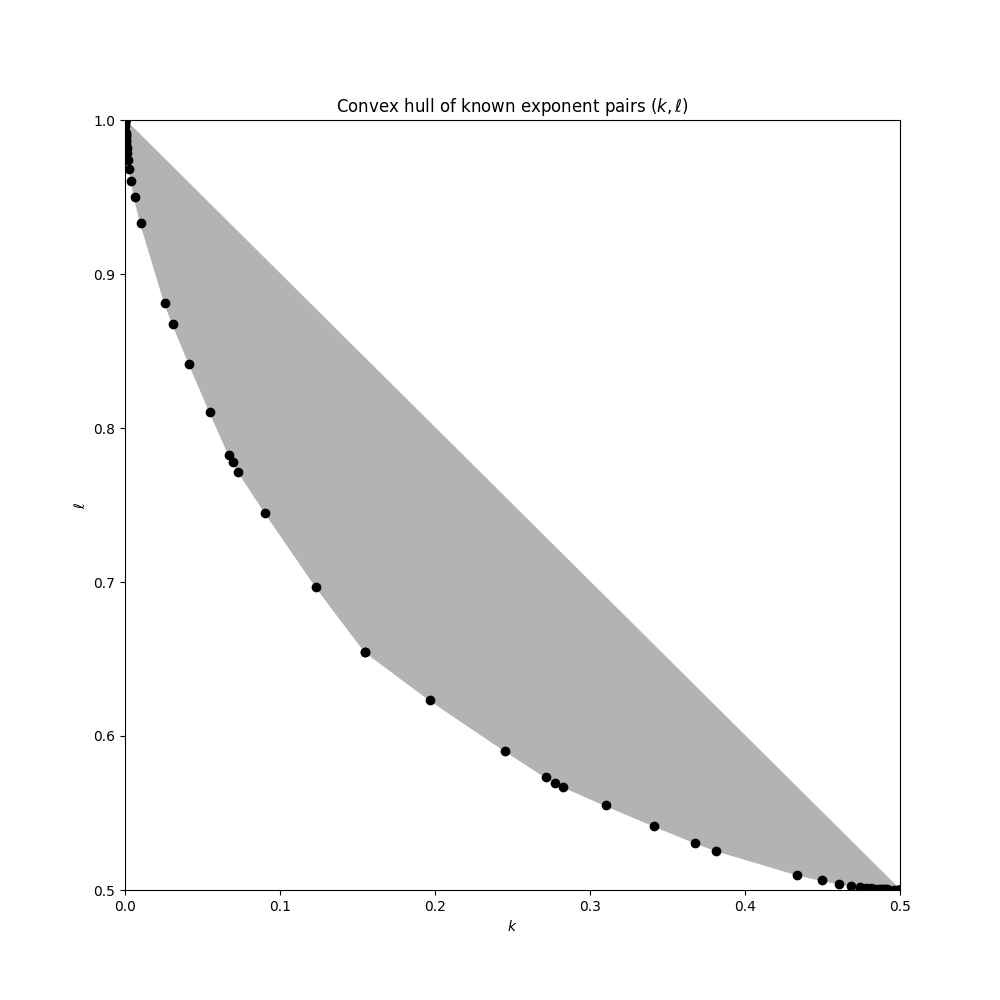
\includegraphics[width=0.5\linewidth]{chapter/exp_pair_plot.png}
    \caption{The convex hull of known exponent pairs, whose vertices $(k_n, \ell_n)$ are given in Table \ref{exp_pair_table}.}
    \label{fig:exp_pair_plot}
\end{figure}
